\section{Teststrategie}
\label{section:Teststrategie}
Om de kwaliteit van het product te waarborgen is er een test strategie opgesteld.
De testen worden gebruikt om de technische en functionele correctheid van het programma aan te tonen.
Dit wordt gedaan door gebruik te maken van het V-Model \parencite{VModel} (zie figuur \ref{fig:VModel}).
Het V-Model is een variatie van de SDLC waar bij er bij elke stap van het proces testen worden uitgevoerd om de kwaliteit van het product te waarborgen.

\whitespace
\begin{graphic}
    \captionsetup{type=figure}
    \caption{V-Model \parencite{VModel}}
    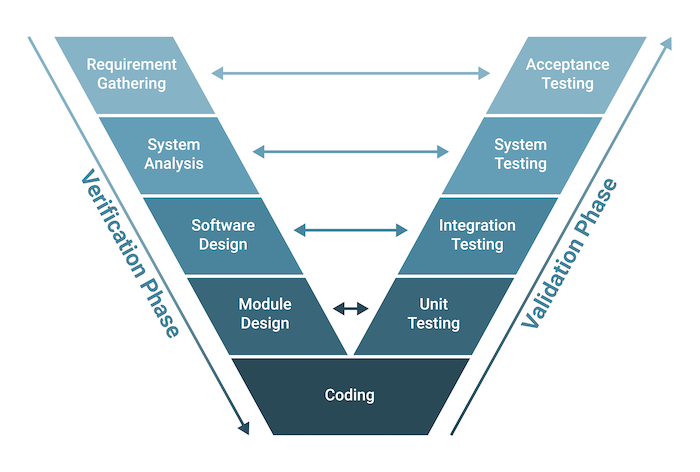
\includegraphics[scale=0.4]{V-model.png}
    \label{fig:VModel}
\end{graphic}

\whitespace
Bij elke stap van de validatie fase van het realiseren worden de verschillende testen uitgevoerd.
De Unit en intergration testen worden automatisch uitgevoerd.
De systeem en acceptatie testen worden met de hand uitgevoerd.
